
%% The first command in your LaTeX source must be the \documentclass command.
\documentclass[manuscript,screen,review,acmsmall]{acmart}

%%
%% \BibTeX command to typeset BibTeX logo in the docs
\AtBeginDocument{%
  \providecommand\BibTeX{{%
    \normalfont B\kern-0.5em{\scshape i\kern-0.25em b}\kern-0.8em\TeX}}}

%% Rights management information.  This information is sent to you
%% when you complete the rights form.  These commands have SAMPLE
%% values in them; it is your responsibility as an author to replace
%% the commands and values with those provided to you when you
%% complete the rights form.
\setcopyright{acmlicensed}
\copyrightyear{2024}
\acmYear{2024}
\acmDOI{XXXXXXX.XXXXXXX}

%% These commands are for a PROCEEDINGS abstract or paper.
\acmConference[CSCW '25]{Make sure to enter the correct
  conference title from your rights confirmation emai}{Oct 18--22
  2025}{Bergen, Norway}
\acmISBN{978-1-4503-XXXX-X/18/06}


%%\citestyle{acmauthoryear}

%%
%% end of the preamble, start of the body of the document source.
\begin{document}

%%
%% The "title" command has an optional parameter,
%% allowing the author to define a "short title" to be used in page headers.
\title{Interlocks Mitigate Information Cascades in Large-Scale Social Learning}

%%
%% The "author" command and its associated commands are used to define
%% the authors and their affiliations.
%% Of note is the shared affiliation of the first two authors, and the
%% "authornote" and "authornotemark" commands
%% used to denote shared contribution to the research.
%\authornote{Both authors contributed equally to this research.}
\author{Authors redacted for peer review}
%\author{Edward L. Platt}
%\email{ed@elplatt.com}
%\orcid{0000-0003-2148-3841}
%\affiliation{%
%  \institution{Cinder Oak}
%  \city{Ann Arbor}
%  \state{Michigan}
%  \country{USA}
%}
%\affiliation{%
%  \institution{University of Michigan}
%  \city{Ann Arbor}
%  \state{Michigan}
%  \country{USA}
%}

%\author{Herminio Bodon}
%\orcid{0009-0004-3270-3621}
%\email{HerminioBodon2020@u.northwestern.edu}
%\affiliation{%
%  \institution{Northwestern University}
%  \city{Evanston}
%  \state{Illinois}
%  \country{USA}
%}
%\affiliation{%
%  \institution{University of Michigan}
%  \city{Ann Arbor}
%  \state{Michigan}
%  \country{USA}
%}

%\author{Daniel M. Romero}
%\orcid{0000-0002-8351-3463}
%\affiliation{%
%  \institution{University of Michigan}
%  \city{Ann Arbor}
%  \state{Michigan}
%  \country{USA}}
%\email{drom@umich.edu}


%%
%% By default, the full list of authors will be used in the page
%% headers. Often, this list is too long, and will overlap
%% other information printed in the page headers. This command allows
%% the author to define a more concise list
%% of authors' names for this purpose.
%\renewcommand{\shortauthors}{Platt, Bodon, \& Romero}

%%
%% The abstract is a short summary of the work to be presented in the
%% article.
\begin{abstract}
Large-scale participatory decision-making is notoriously difficult, but successful examples have recently become more common. These examples have been enabled in-part by the fast, affordable, many-to-many communication afforded by the internet. But not all large-scale participatory projects on the internet are successful. We review the empirical literature on successful large-scale participatory projects and identify a common feature: interlocking network structure. We use agent-based modeling to simulate the effects of interlocking network structure on large-scale social learning. We find that in high-conformity contexts, interlocks can provide a protective effect against information cascades and polarization. Our findings suggest that interlocking network structure is beneficial for large-scale participatory projects, and we identify likely mechanisms behind that benefit.
\end{abstract}

%%
%% The code below is generated by the tool at http://dl.acm.org/ccs.cfm.
%% Please copy and paste the code instead of the example below.
%%
\begin{CCSXML}
<ccs2012>
<concept>
<concept_id>10002950.10003624.10003633</concept_id>
<concept_desc>Mathematics of computing~Graph theory</concept_desc>
<concept_significance>500</concept_significance>
</concept>
<concept>
<concept_id>10003120.10003130.10003131.10003570</concept_id>
<concept_desc>Human-centered computing~Computer supported cooperative work</concept_desc>
<concept_significance>500</concept_significance>
</concept>
<concept>
<concept_id>10010147.10010341.10010349.10010355</concept_id>
<concept_desc>Computing methodologies~Agent / discrete models</concept_desc>
<concept_significance>300</concept_significance>
</concept>
</ccs2012>
\end{CCSXML}

\ccsdesc[500]{Mathematics of computing~Graph theory}
\ccsdesc[500]{Human-centered computing~Computer supported cooperative work}
\ccsdesc[300]{Computing methodologies~Agent / discrete models}


%%
%% Keywords. The author(s) should pick words that accurately describe
%% the work being presented. Separate the keywords with commas.
\keywords{Collaboration, Social Learning, Networks, Interlocks, Information Cascades, Polarization, Deliberation, Consensus}

\received{29 October 2024}

%%
%% This command processes the author and affiliation and title
%% information and builds the first part of the formatted document.
\maketitle

\section{Introduction}
Large collaborations face a dilemma:
participatory governance is both
highly desirable and notoriously difficult
to implement in large groups.
Elinor Ostrom's empirical study of commons governance identified participatory rule-making
as one of the key principles necessary for the success and longevity of resource regimes
\cite{ostrom_collective_2000, ostrom_governing_1990}.
Participatory governance, particularly participatory deliberation,
enables the aggregation and synthesis of diverse knowledge
\cite{
dewey_creative_1940,
anderson_epistemology_2006,
ackerman_deliberation_2002},
benefits from the wisdom of crowds
\cite{
surowiecki_wisdom_2005,
hill_group_1982,
hong_groups_2004,
golub_naive_2010,
galton_vox_1907},
identifies and resolves conflicts
\cite{gentry_consensus_1982},
and incentivizes future cooperation by increasing perceptions of trust and fairness
\cite{
ostrom_collective_2000,
bowles_endogenous_1998}.
Unfortunately, as groups grow larger so does the difficulty of participatory governance.
The challenges of participatory governance in large groups include:
increased time and effort needed to reach decisions
\cite{
fishkin_voice_1997,
gentry_consensus_1982,
steiner_group_1972},
the emergence of power inequalities
\cite{
freeman_tyranny_1972,
shaw_laboratories_2014,
kittur_power_2007,
boehm_egalitarian_1993},
and counterproductive social dynamics such as
information cascades \cite{banerjee_simple_1992},
polarization \cite{schkade_what_2007},
social loafing \cite{karau_social_1993},
and the majority illusion \cite{lerman_majority_2015}.
Yet examples of successful large-scale participatory governance do exist, including Wikipedia \cite{giles_internet_2005, keegan_evolution_2017, forte_scaling_2008}, free and open source software projects \cite{benkler_coases_2002}, grassroots protest and crisis-response networks \cite{manilov_occupy_2013, tufekci_twitter_2017,
gonzalez-bailon_networked_2016,
landau_place-based_2017,
brugh_combining_2019}
and self-managed organizations
\cite{laloux_reinventing_2014,monsen_buurtzorg_2013,robertson_holacracy_2015}.
These examples often rely on the unprecedented fast, inexpensive, many-to-many communication afforded by the internet.
But not all internet-enabled participatory collaborations succeed \cite{tufekci_twitter_2017, geiger_does_2009}. Why do some succeed while others fail?

In this paper, we begin with a review of the literature on large-scale participatory decision-making and related topics.
We focus, in particular, on empirical studies of successful large-scale participatory projects, looking for commonalities.
We then focus on one such commonality: social network structure,
specifically a type of network known as an interlock network.
We also narrow our focus to social learning:
the process by which individuals revise their beliefs and opinions
based on observations and interactions with others---a core part of participatory decision-making.
Finally, we develop an agent-based model
to test the effects of interlock networks on social learning
in large groups.
Our findings suggest that interlock network structure may contribute to the success of large-scale participatory projects by providing protection from information cascades and polarization.

\subsection{Empirically-Motivated Simulation}

If large-scale participatory decision-making is difficult,
then studying it is doubly so.
The large number of individuals involved makes lab experiments prohibitively expensive.
Randomized, controlled field experiments would require dividing
a community into control and treatment arms
and ensuring that the members of each
arm do not interact,
which is both impractical and potentially
against the best interests of the group members,
especially if they are making consequential decisions.
For the present study, we use computer simulation models to help bridge the gap
between empirical observation and future experimentation.

Readers may understandably question how well a computer simulation can provide insight into the rich complexities of human behavior.
As with all models, computer and otherwise,
the usefulness of our methodology depends on the soundness of our simplifying assumptions and the applicability of our outcome measures.
So we base both on a thorough review of the observational literature.
If our model finds that the conditions present in real-world participatory groups lead to the outcomes observed in real-world participatory groups,
we can provide insight into how and why those conditions might lead to those outcomes.

Specifically, we use Agent-Based Modeling (ABM),
well-established type of simulation model often used in complex systems,
economics, and biology
\cite{hong_groups_2004,
lazer_network_2007,
golub_naive_2010,
zollman_social_2012,
grim_scientific_2013,
barkoczi_social_2016,
gomez_clustering_2019}.
Simply put, we simulate a large number of agents, each modeling a single group participant.
We allow those agents to interact based on well-defined behavioral strategies,
and observe the progression of their states over time.
We describe our model in greater detail in
Sections \ref{subsec:abm}---\ref{subsec:nk} and \ref{sec:methods}.
Our empirically-motivated simulation approach allows us to isolate individual factors and perform controlled experiments with a precision and scale not feasible in a real-world setting, while remaining grounded in real-world observations.
Our findings can establish the plausibility of empirically-motivated hypotheses,
provide insight into the underlying mechanisms,
and provide guidance and motivation for future real-world empirical studies.

\subsection{Collaboration and Network Structure}
As we will elaborate below,
we find that real-world examples of successful large-scale participatory collaborations
often share a common trait:
interlocking social network structure.
Here, we use ``network'' in the sense of a set of entities with dyadic relationships between them \cite{newman_networks_2018}, e.g.,
individuals linked to other individuals through direct communication.
Similarly, we use ``structure'' to refer to the configuration of individual dyadic relationships and connections, rather than in the systemic or institutional sense. A roundtable discussion for example,
is structured to allow communication links between any pair of indidividuals, while a lecture has links from the lecturer to the audience but not between audience members (at least if they are polite).
An {\em interlocking network} or {\em interlock}
is a network in which groups of entities are connected (interlocked)
through shared individual constituents \cite{taylor_world_2015}.
As a much-studied example,
an interlocking directorate is a network of corporations
in which two corporations (the groups) are considered connected if any individual director (the constituent) belongs to both of their boards 
\cite{mizruchi_what_1996}.
Or as a more modern example,
collaborative interactions on Wikipedia take place on individual articles, their per-article talk pages, and on topical WikiProject pages \cite{platt_network_2018}.
In this example, articles/talk pages/projects are the groups, and individual editors are the constituents.

The relationship between network structure and large-scale participatory collaboration may not be immediately obvious.
In large collaborations, while it may be the case that anyone {\em can} talk to anyone else, it is not the case that everyone {\em does} talk to everyone else.
The number of potential interactions is much greater than the capacity of the collaborators.
This fact implies a network structure: who interacts with whom.
While hierarchical ``tree'' networks are a practical way to interconnect a large group of people,
as in a military chain of command or corporate org chart,
they privilege some group members above others.
Participatory collaboration requires different structures.
In the context of self-organized collaboration, most network-based analyses have focused on 
small-world networks \cite{watts_collective_1998}
and preferential attachment networks \cite{barabasi_emergence_1999},
rather than interlocks,
with the notable exception of Salehi \& Bernstein's work on network rotation \cite{salehi_hive:_2018}.

There is considerable evidence that group composition
\cite{hill_group_1982,
nishi_inequality_2015,
robert_jr_differences_2018,
sydow_diversity_2017,
lerner_diverse_2018,
arazy_information_2011}
and social network structure
\cite{
kearns_experiments_2012,
barkoczi_social_2016,
salehi_hive:_2018,
mason_propagation_2008,
mason_collaborative_2012}
can influence the success of a collaboration.
Interlocking structure has implications for both of these factors.
By dividing an entire collaborative project into smaller groups,
interlocks reduce group size and alter group composition,
potentially sidestepping some of the pitfalls of large group collaboration.
For example, a participant who monoplizes the conversation might derail their small group, but not the entire project.
Or, a member of an underrepresented demographic would have more chances to speak as a participant in a small group of five versus a large group of one hundred.
Additionally, by creating interconnections between groups through mutual membership,
interlocks influence the overall structural properties of the network.
In turn, those structural properties influence the speed and flow of information diffusion through the entire population of collaborators.

\subsection{Social Learning}
To begin to disentangle the multiple ways interlocking structure might influence the large participatory collaborations,
we focus on a subset of possible factors.
Specifically, we model collaborations as {\em social learning} processes \cite{barkoczi_social_2016, mason_collaborative_2012, hong_interpreted_2009, degroot_reaching_1974},
in which homogeneous agents exchange information and choose preferred solutions to a problem based on a combination of individual assessments of solution quality and information received from peers.
In this model, agents can apply different
{\em social learning strategies} to integrate socially acquired information with their own individual assessments.
Strategies can be classified as {\em high-connformity} when social influence is prioritized over individual assessments and {\em low-conformity} in the opposite case.
While this model leaves out many real-world collaborative considerations,
ranging from the deep
(e.g.,
argumentation \cite{fishkin_voice_1997, mansbridge_minimalist_2015},
identity \cite{bail_breaking_2022,schkade_what_2007},
implicit bias \cite{amodio_stereotyping_2006},
interpersonal conflict\cite{whiting_did_2019})
to the mundane (e.g.,
mood, 
conversational tone),
solution-quality-based considerations are common across collaborations,
and are considered by many scholars to be a normative or even necessary
part of participatory decision-making
\cite{mansbridge_minimalist_2015}.
We thus propose this work as an starting point for understanding the seemingly-important role of interlocks in large-scale participatory collaboration, leaving additional considerations as crucial future work.

\subsection{Research Questions}
Our primary focus is whether interlocking network structure is beneficial for social-learning-based collaboration:
\begin{quote}
{\bfseries RQ 1.} Does interlocking structure influence solution quality in large-scale social learning?
\end{quote}

As higher quality collaborative output has sometimes been observed to require longer spans of time
\cite{
gentry_consensus_1982,
platt_network_2018},
we also ask whether interlocking structure
has any such influence:

\begin{quote}
{\bfseries RQ 2.} Does interlocking structure influence speed of convergence in large-scale social learning?
\end{quote}

Social learning strategies have been shown to modulate the influence of network structure on collaborations
\cite{barkoczi_social_2016, zollman_social_2012},
so we also ask whether the same is true for the effects of interlocking networks:

\begin{quote}
{\bfseries RQ 3.} Are the effects of interlocking structure on social learning modulated by social learning strategy?
\end{quote}

Finally, as polarization is one of the mechanisms known to hinder quality in social learning and collaboration
\cite{schkade_what_2007, zollman_social_2012},
we ask whether interlocking network strucutre has an effect on polarization:

\begin{quote}
{\bfseries RQ 4.} Does interlocking structure influence polarization in large-scale social-learning?
\end{quote}

\subsection{Contributions}
In this paper, we present the following contributions:
\begin{itemize}
\item{We show that social-learning on interlocks outperforms small-world and preferential attachment networks for some social learning strategies, and performs comparably for others (RQ 1).}
\item{Specifically, we show that in groups using a conformist social learning strategy, interlocks outperform other networks (RQ 3).
We attribute this improvement to a protective effect against information cascades that lead to the adoption of popular but sub-optimal solutions.}
\item{We also show that interlocks do not result in notably slower convergence, even in cases where they improve solution quality (RQ 2).}
\item{Finally, we show that interlocks reduce polarization when agents are using a conformist strategy (RQ 4).
Again, we attribute this result to a protective effect against information cascades.}
\end{itemize}
Taken together, our findings show that interlocks provide a protective effect against information cascades in large-scale social learning, which improves the performance of high-conformity strategies while resulting in similar performance for low-conformity strategies.
This protective effect may contribute to the relative success observed in large participatory collaborations with interlocking network structure.

\section{Background}

Examples of large participatory collaborations have become increasingly common in recent years,
and some have achieved surprising levels of success.
In particular, many of these recent successes rely on the fast, inexpensive, many-to-many communication afforded by the internet,
which has enabled an environment Jochai Benkler calls the ``networked information economy''
\cite{benkler_wealth_2006}.
Wikipedia, the popular online encyclopedia has been produced by millions of editors (47.6 million for just the English language edition at time of writing \cite{noauthor_list_2024, noauthor_wikipediawikipedians_2024})
using consensus-based, participatory decision-making \cite{keegan_evolution_2017, forte_scaling_2008}.
Despite common wisdom regarding the impossibility of large-scale participatory governance,
Wikipedia has been found comparable in quality to traditionally-edited encyclopedias \cite{giles_internet_2005},
leading to the popular Wikipedian in-joke that
``The problem with Wikipedia, is that it only works in practice. In theory, it's a total disaster'' \cite{elsharbaty_editing_2016}.
Similarly, Free and Open-Source Software (FOSS),
which is also highly participatory,
has achieved a level of success that rivals traditionally-produced software
\cite{benkler_wealth_2006, raymond_cathedral_1999}.
As one example, the FOSS operating system Linux is the most popular OS for internet servers and the core of the Android OS for mobile devices.
In a business context, examples of participatory worker self-management can be found in both corporate and cooperative contexts \cite{laloux_reinventing_2014, lee_self-managing_2017}.
Examples include Zappos.com's evolving use of the Holacracy system
\cite{robertson_holacracy_2015, groth_zappos_2020}
and the Buurtzorg model of homecare
\cite{monsen_buurtzorg_2013, gray_home_2015}.
Grassroots social movements and crisis-response groups have also made use of participatory governance.
The Occupy movement embraced participatory governance \cite{detar_intertwinkles:_2013, gonzalez-bailon_networked_2016}
which resurfaced in the 60,000 self-organized volunteers of the Occupy Sandy crisis-response efforts \cite{landau_place-based_2017, brugh_combining_2019}.
Similarly, participatory practices were a key part of the 2013 Gezi Park protests
\cite{tufekci_twitter_2017}.

\subsection{Interlocks\label{subsec:interlocks}}
When reviewing these examples, a remarkably common pattern stands out: interlocking network structure.
In these successful examples of large-scale participatory projects,
communication is frequently organized into small participatory groups of peers based on interest, region, function, or simply happenstance.
These groups are then interconnected through individuals who participate in multiple groups.
We reproduce excerpts from several examples here to demonstrate the ubiquity of this pattern.

Occupy Wall Street and Occupy Sandy \cite{manilov_occupy_2013}:
\begin{quote}
One of the greatest strengths of the Occupy movement has been its willingness to decentralize decision-making into networks built on a foundation of small groups that move easily between online and real-world activities.
\end{quote}

The 2013 Gezi Park protests in Turkey \cite{tufekci_twitter_2017}:
\begin{quote}
The next day, the protesters at the park initiated a ``small-forum'' process,
inviting people to break into small groups to discuss the government’s proposal. 
\end{quote}

Blogs on the early web \cite{benkler_wealth_2006}:
\begin{quote}
Filtering, accreditation, synthesis, and salience are created through a system
of peer review by information affinity groups, topical or interest based.
These groups filter the observations and opinions of an enormous range of people,
and transmit those that pass local peer review to broader groups and ultimately to the polity more broadly...
\end{quote}

US anti-war protests \cite{detar_intertwinkles:_2013}:
\begin{quote}
The core of these protests were
organized by clusters of small-scale affinity groups. Each affinity
group, consisting of 10 to 20 people, decided what sort of role they
were comfortable fulfilling, and then coordinated with other affinity
groups to participate in larger actions.
\end{quote}

Collaborative design \cite{salehi_hive:_2018}:
\begin{quote}
We argue that large
collectives cannot cross-pollinate ideas simply by placing all ideas into the commons for others to
see — people in the collective must instead interact with each other closely to benefit from ideas and
perspectives that each bring to the table.
We define an approach, network rotation, that supports
this goal by gradually weaving together team membership from across the collective to increase
the efficiency of the underlying collaboration network while maintaining high tie strength within
teams.
\end{quote}

The above examples all share the same social network structure of small groups connected through mutual membership: {\em interlocks}.
Interlocks have been well-studied in several other contexts.
Perhaps the most well-known is the study of intelocking directorates,
the practice of one individual sitting on the board of directors for
multiple corporations,
allowing an implicit flow of information and influence
\cite{sapinski_interlocking_2018}.
Interlocks arise in other fields as well,
including revolutionary cells
\cite{fischer_paul_1994, healy_using_2013},
the UK suffragette movement \cite{crossley_covert_2012},
and the global network of cities \cite{taylor_world_2015}.

\subsection{Participatory Governance and Social Learning}
This paper touches on several related topics, namely: problem-solving, decision-making, deliberation, and social learning.
These concepts are very closely related, but not equivalent,
potentially leading to confusion.
Matters are made worse by differing (and conflicting) definitions in the literature.
Here, we attempt to untangle this conceptual knot.

The motivation and ultimate focus of our work is {\em participatory governance}
in the sense Elinor Ostrom's third design principle for long-suriving resource regimes: that ``most of the individuals affected by a resource
regime can participate in making and modifying their rules.''
\cite{ostrom_collective_2000}
In this sense, governance is largely about {\em decision-making} regarding
rules and their enforcement.
But we are careful to note that rules and decisions can implicit
{\em rules-in-use} in addition to explicit {\em rules-in-form}
\cite{hess_framework_2005, keegan_evolution_2017}.

\subsubsection{Deliberation}
{\em Deliberation} is an exemplar of participatory governance.
But prior to the internet and other forms of digital communication,
the logistics of large-scale governance generally excluded more participatory
forms of decision-making \cite{ackerman_deliberation_2002}.
More tractable alternatives such as voting and representative
assemblies are less participatory.
There is no consensus on the exact definition of deliberation.
We will follow the ``minimalist'' definition proposed by Dryzek
\cite{dryzek_deliberative_2002} and refined by Mansbridge \cite{mansbridge_minimalist_2015}:
\begin{quote}
Deliberation is mutual communication that involves weighing and reflecting on preferences, values and interests regarding matters of common concern.
\end{quote}
Note that this definition does not actually require the making of a decision, but by explicitly mentioning ``preferences," does imply the existence of a decision to be considered.
And again, while ``deliberation'' may conjure images of formal institutions,
note that the above definition includes both formal and informal communication,
as long as it is mutual and non-coercive.

\subsubsection{Social Learning\label{subsec:social}}
In {\em social learning}, individuals revise their beliefs by observing and interacting with others.
Social learning allows an individual to augment their limited information and perspective by observing others who may have different information
and perspectives \cite{hong_interpreted_2009, golub_naive_2010}.
When this observation takes the form of mutual communication,
social learning fits nicely into the above definition of deliberation.
In fact, many models of social learning implicitly assume mutual communication
\cite{golub_naive_2010, lazer_network_2007, mason_collaborative_2012, barkoczi_social_2016, gomez_clustering_2019}.
Deliberation is a thus a type of social learning,
and the results from the above models should be expected to apply.

Why do people engage in social learning?
Usually to solve problems.
Specifically, to solve problems too complex or resource-intensive to
solve individually.
In other words, social learning is also a form of collective
problem-solving and collective intelligence.
Participatory governance is such a problem.

In the case of participatory governance,
there are two related, but subtly different problems being solved.
The first problem is for participants try to accurately determine which outcome would maximize social utility.
For example, a group deciding what type of pizza to order might gather information on other participants' most and leaast favorite pizza toppings.
The second problem is for participants to
advocate for their desired outcome,
which might be based on their personal preference
or on the expected social utility,
e.g., arguing for their favorite pizza topping
or for a pizza topping they believe will satisfy the most people.
The former problem is a matter of information and mathematics,
while the latter is a matter of taste and rhetoric.
Matters of taste are beyond our methods, so our models focus on the former problem of gathering information and maximizing utility.
So we model a group's ability to identify outcomes that maximize
common good.
This is a necessary, but not sufficient condition for the group to actually
adopt such an outcome.

\subsubsection{Putting It All Together}
Summarizing the above, we use an agent-based model to simulate a group's
ability to collectively problem-solve
---
through the use of mutually-communicative,
deliberation-like social learning
---
the problem of fidning a governance outcome that maximizes the social utility of the group.
To the extent that a group prioritizes such outcomes,
our models should provide meaningful insight.

\subsection{When Social Learning Goes Wrong}
While social learning can allow members of a group to combine their knowledge and resources,
it can also introduce new problems.
When information is repeated without sufficient independent checking,
a false belief starting with one person can be repeated and amplified until it is accepted by a large number of people:
an {\em information cascade} \cite{banerjee_simple_1992}.
Similarly, in the {\em majority illusion},
an individual may incorrectly infer that the majority of a group holds a particular belief if they are only exposed to others who do hold that belief \cite{lerman_majority_2015}.
Finally,
rather than reaching a single consensus,
social learning can cause {\em polarization},
in which a group fragments into two or more factions which hold similar beliefs within each group,
but conflicting beliefs between groups
\cite{schkade_what_2007}.
In groups that successfully implement large-scale participatory decision-making,
these pitfalls must be avoided.
One of this paper's main goals is to identify potential structural or behavioral mechanisms that might allow a group to do so.

\subsection{Agent-Based Modeling\label{subsec:abm}}
Our Agent-Based Model (ABM) closely follows previous ABM work on social learning
\cite{lazer_network_2007, barkoczi_social_2016, gomez_clustering_2019}.
The ABM consists of a large collection of {\em agents}:
simulated entities, each with their own private information and the ability to update that information based on interactions with other agents.
In our case, the agents are intended to represent
individual participants in a participatory decision-making
process.
The exact behavior of the agents is determined by three factors:
\begin{description}
\item[Objective Function]
At the beginning of each ABM run, an objective function $Q(s)$ is defined.
The goal of the agents is to find an $s$ that maximizes
$Q(s)$.
\item[Social Network]
The social network provides links between some pairs of agents and not others.
These links allow neighboring agents to interact with each other and share information.
\item[Social Learning Strategy]
The social learning strategy is a simple set of rules the agents use to interact with their neighbors and update their belief about the best value of $s$.
\end{description}

At the beginning of a simulation run, each agent is initialized with a random $s$.
The run proceeds in discrete time steps.
At each time steps, each agent interacts with each of its neighbors according to its strategy and
updates its belief.
After a fixed number of time steps, the run ends.
Ideally, the number of time steps is large enough that
the agents' beliefs have reached a stable state.
Different agents may still have different beliefs,
but at this point the distributions of beliefs and the potential outcomes of votes can be analyzed.
This process is repeated for many runs,
each with a new set of initial conditions and objective $Q(s)$.
By performing many runs, statistical differences between different networks and/or strategies can be identified.

\subsection{NK Model\label{subsec:nk}}
For our agent-based model, we need an objective function $Q(s)$ for the agents to maximize.
We follow previous literature on social learning
\cite{lazer_network_2007,barkoczi_social_2016,gomez_clustering_2019}
by using the NK Model \cite{kauffman_towards_1987,weinberger_local_1991} to create our objective function.
The NK Model has a number of properties that make it a good candidate for modeling social learning.
It was originally developed to model the natural selection of genetic mutations \cite{kauffman_towards_1987},
but we describe it below in terms of a more relevant example.

Let's consider a referendum on $N$ different yes/no proposals.
These proposals might, for example, be of the following sort:
\begin{itemize}
    \item{Should a new housing development be approved at 123 Main Street?}
    \item{Should electric scooters be permitted on sidewalks?}
    \item{Should a traffic lane be added to Anytown Highway?}
\end{itemize}

Individuals may feel strongly about some of the proposals and not at all about others.
Rather than considering individual voters, let's consider voting blocs:
groups of people who are all concerned about the same issues.
Specifically, let's assume that there are $N$ voting blocs, each mostly concerned with one of the $N$ proposals.
However, the result of implemenmting any single proposal might depend on which of the other propsals are implemented.
One bloc for example, let's call them the {\em Bloc for Beds, Bikes, and Busses}, might support approving new a housing development,
but only if additional public transportation and bike lanes are created.
So we also assume that each bloc is concerned with $K$ additional proposals, for a total of $K+1$.

After the vote is held and the results have been implemented, each bloc $n$ will have some approval rating $q_n(s)$,
where $s$ is an $N$-bit binary number with each bit representing the outcome of one yes/no proposal.
Each bloc's approval rating will depend on the outcomes of the $K+1$ relevant proposals.
Note that we don't need to assume that the voters themselves know or can predict ahead of time what their approval rating for each possible outcome would be.
By averaging the approval ratings of each bloc for a given outcome $s$, we get a number representing the social utility, fitness, or {\em quality} of that solution:
\begin{eqnarray}
    Q(s) &=& \frac{1}{N}\sum_{n=1}^N q_n(s).
\end{eqnarray}
Any such function $Q(s)$ is an instance of the NK Model.

In this paper, as is typical with the NK Model, we determine the $q_n$ randomly.
First by chosing the relevant $K$ bits of the solution at random, and then by assigning a uniform random value in [0,1] $q_n$ for each possible input.
Random $q_n$ are suitable when we care more about how agents incorporate information about preferences than about why those preferences exist in the first place.

\subsubsection{The NK Model in Participatory Decision-Making}
The above description uses the language of proposals, voting blocs, and approval ratings. This language should not necessarily be taken literally.
We have used it to motivate the NK Model as a suitable model for complex policy decisions.
However, the NK model is just as applicable to a situation where, for example, the "voting blocs" are farm crops, the "policies" are farming practices, and the "fitness" is the crop yield; or to genes, mutations, and reproduction rates, as in the original conception of the NK Model \cite{kauffman_towards_1987}.

We draw attention to the above distinction because of a subtle, but very important point.
As discussed in Section \ref{subsec:social} there are two related but separate approaches to participatory governance.
One, to advocate for a preferred outcome based on preferences;
the other, to determine which outcome would best satisfy everyone's preferences.
The NK Model bridges these two approaches.
It asks: given a random set of subjective preferences,
what is the objective quality of a particular outcome?

\subsubsection{Properties of the NK Model}
The real-world applicability of our findings will depend on how well a real-world system agrees with the assumptions of our model.
We enumerate key assumptions and properties below.
\begin{description}
\item[Discrete solution space]
The NK model solution space consists of discrete states.
This space best represents a set of yes/no questions.
However, the NK model can also be applied to any solution space that can be approximated by a discrete set of solutions, for example, by dividing a continuous range into bins.
\item[Large solution space]
There are $2^N$ possible solutions for any particular instance of the NK model.
The number of solutions grows exponentially with the number of bits in $s$.
The NK model is thus well-suited to representing problems with far more potential solutions than could ever be evaluated.
For example, for N=33, there would be more potential solutions than humans alive on Earth (at time of writing).
\item[Rugged solution space]
Often called a ``rugged landscape,'' the NK model has many local maxima and minima,
often described as ``peaks'' and ``valleys.''
A simple hill-climbing search by changing one solution bit at a time will lead to a local maximum,
but there is no way to know if a better solution exists, other than searching for it.
This is a common (if frustrating) feature of real-world problems.
\item[Tunably rugged]
In addition to being rugged, the ruggedness of the NK model can be ``tuned'' by changing the $K$ parameter.
For a value of $K=0$, each solution bit can be optimized independently, and there is a single local maximum.
For the maximum value of $K=N-1$,
the landscape is essentially random.
For intermediate values of $K$,
there are a large number of local maxima, but they are surrounded by ``basins of attraction'' which allow those maxima to be found from nearby solutions using hill-climbing.
These intermediate values are typically the ones used to mimic real-world rugged landscapes.
\item[NP-complete]
For $K \geq 3$, the problem of finding the global optimum of the NK model in general is NP-complete \cite{weinberger_np_1996}.
This means that the NK model is computationally equivalent to the hardest problems solvable by a computer,
and can thus model the complexity of any problem that is capable of being modeled computationally.
\end{description}

\subsection{Social Learning Strategies}
The behavior of agents is defined by a {\em social learning strategy}.
These strategies are sets of rules that instruct an agent how to interact
with its neighbors and how to update its beliefs based on that interaction.
Different social learning strategies model different real-world behaviors.
They also make different assumptions about the capabilities of agents to
evaluate their own beliefs and the beliefs of their neighbors.
In this paper we follow the strategies defined by Barkoczi and Galesic \cite{barkoczi_social_2016}.

\subsubsection{Best-Neighbor}
The {\em best-neighbor} strategy is a naive, greedy strategy.
Agents simply evaluate the quality of each neighbor's candidate solution,
and adopt the best one.
In general, greedy algorithms are fast and efficient, but often converge
to sub-optimal local maxima.
Note that this strategy also assumes agents are capable of objectively
evaluating which of two solutions is better.
In other words, given two candidate solutions $s$ and $s^\prime$,
they can evaluate whether $Q(s^\prime) > Q(s)$.
Note that this does not require that agents are capable of evaluating
the exact value of $Q(s)$.
Because this strategy prioritizes solution quality over solution popularity,
we calssify it as a {\em low-conformity} strategy.

\subsubsection{Conform}
The {\em conform} strategy is, as its name suggests,
a {\em high-conformity} strategy.
In this strategy, agents survey the solutions of their neighbors and
select the most popular strategy.
Ties are broken randomly.
In the case that no candidate solution has been adopted by more than one
neighbor,
the agent simply keeps its previous candidate.
We also assume the {\em critical learning} convention
\cite{barkoczi_social_2016, rendell_rogersparadox_2010},
in which agents will only adopt a popular candidate solution if it is better
than their own.
This strategy requires that given a candidate solution,
agents are able to determine whether it is objectively better than their own.
However, it does not require the capability to compare the quality of two
{\em arbitrary} candidates.
The conform strategy models real-world settings in which individuals are
unable or uninclined to compare the quality of all options before them,
but can determine whether a single popular option is an imporovement over one
they have experience with.

\subsubsection{Individual}
In addition to social learning, agents may also engage in {\em individual}
learning.
Following \cite{barkoczi_social_2016},
we model individual learning as a hill-climbing algorithm.
Agents try changing a single bit of their candidate solution and determine
whether the new candidate is an improvement.
These strategies represent exploration of incremental improvements on existing
solutions.
Repeatedly applying individual learning will eventually lead to a local
maximum.

\subsection{Network Types}
Once agents have a problem to solve, and a strategy for interacting with
their neighbors, they need to know who their neighbors are.
This section describes the social network topologies used in our model.

\subsubsection{Small-World}
In {\em small-world} networks
\cite{watts_collective_1998},
individuals are mostly linked to others in the
same spatial or geographic location,
but have some long-distance {\em shortcuts}.
The local ties create high {\em clustering}:
an individuals neighbors are likely to be neighbors to each other.
The shortcuts act as weak ties \cite{granovetter_strength_1973},
reducing the ``size'' (mean shortest path length)
of the network by creating short paths
between any two individuals.
High clustering and short path length are often observed in real-world social
networks.
In a $k$-degree Watts-Strogatz small-world network \cite{watts_collective_1998},
individuals are assigned to locations on a ring and connected to their
$k$ nearest neighbors (not to be confused with $K$ from the NK model).
For each of an individuals links,
with a probability $\beta$,
the other end of the link is assigned to a random individual,
creating the shortcut edges.

\subsubsection{Preferential Attachment}
Some real-world social networks exhibit a skewed, heavy-tail degree distribution:
most individuals linked to few others,
but a few ``hubs'' or ``influencers'' linked to many others.
Such networks can be modeled using the Barabási-Albert preferential attachment model
\cite{barabasi_emergence_1999}.
In this model, as individuals are added to a network,
they are randomly linked to $m$ others.
The probability of such links is proportional to the target's degree
(number of existing links),
creating a ``rich-get-richer'' dynamic and a heavy-tailed degree distribution.
These networks model settings where a small number of individuals produce a disproportionate share of the communication due to factors such as social capital, expertise, or confidence.

\section{Methods\label{sec:methods}}

\subsection{Modeling Interlocks: Random-Pod Networks\label{subsec:randompod}}
In addition to the two common models of social networks above,
we also model interlock networks,
the central focus of this paper.
Interlock networks are described in detail in Section \ref{subsec:interlocks},

We model an interlock as a time-dependent network.
For a degree $k$ {\em random-pod network},
each agent is randomly assigned to a ``pod''
such that $k+1$ agents are assigned to each pod.
Agents assigned to the same pod are linked by a network edge,
resulting in a fully-connected clique for each pod.
After some number of time-steps, the pod assignments are re-randomized,
creating new cliques.
The movement of agents between pods over the course of the simulation
creates interlocking structure.

By using a time-dependent network, we are able to specify the degree (number of neighbors) of each agent at any given time.
This allows us to choose all of our networks to have the same mean degree,
reducing potential counfounding effects.

The random-pod network model is similar to Salehi and Bernstein's network rotation
\cite{salehi_hive:_2018}.
The key difference is that in network rotation,
pods are changed by a single member at a time, while the random-pod network
reassigns all members simultaneously.
We opt for simultaneous reassignment because it best represents interlock networks
with multiple membership in distinct groups.

\subsection{Agent-Based Model Parameters}
We simulate social-learning using an Agent-Based Model (ABM) closely resembling those of other authors \cite{
lazer_network_2007,
barkoczi_social_2016,
gomez_clustering_2019}.
For our model, we simulate 100 agents.
Each agent maintains a solution candidate and updates that candidate
at each time step according to its learning strategy.
Within each run, all agents use the same learning strategy.
Each run is simulated for 300 time steps
(we have found this is sufficient to achieve convergence for our paremeters).
We created 1000 random instances of the NK model.
For each instance, we simulated each combination of network and learning strategy.

\subsubsection{Objective Function}
Agents search for a binary string $s$ that maximizes an objective
function $Q(s)$ defined by the NK model \cite{kauffman_towards_1987, weinberger_local_1991}.
In keeping with other authors \cite{lazer_network_2007, barkoczi_social_2016}, we use $N=15$, $K=6$.
We also follow the common practice of raising the raw NK fitness to a power of 8
to emphasize peaks and valleys: $Q(s) = Q_{NK}(s)^8$.
Similarly, we normalize fitness values to the global maximum.

\subsubsection{Network}
Agents are placed on a network with the vertices representing
the agents, and edges representing which agents can interact.
We use three separate network topologies:
\begin{description}
    \item[Small-World:]{A 4-degree Watts-Strogatz small-world network with $\beta = 0.1$;}
    \item[Preferential Attachment:]{A Barabási-Albert network with $m=2$ (mean degree 4);}
    \item[Random-Pod:]{A 4-degree random-pod network.}
\end{description}

\subsubsection{Learning Strategy}
At each time step, agents perform individual learning on their previous
solution candidate, followed by one of two social learning strategies:
\begin{description}
\item[Best-Neighbor]{(low-conformity)},
\item[Conform]{(high-conformity)}.
\end{description}

\section{Results}

\subsection{Interlocks and Solution Quality}
Figure \ref{fig:quality} shows the distribution of solution quality over
the 1000 simulation runs.
The quality shown is averaged over the ending solutions of all 100 agents.
For the low-conformity best-neighbor strategy,
all network topologies perform comparably.
For the conform strategy however,
both the small-world and preferential attachment networks
perform notably worse, while the random-pod network actually performs
very slightly better.
It is not surprising that the small-world and preferential attachment networks
show reduced solution quality in a high-conformity settings.
In such settings, it is well-known that information cascades can lead to the adoption of initially popular but sub-optimal solutions
\cite{banerjee_simple_1992}.
So it is remarkable that the random-pod network does not show this behavior.

\begin{figure}
\begin{center}
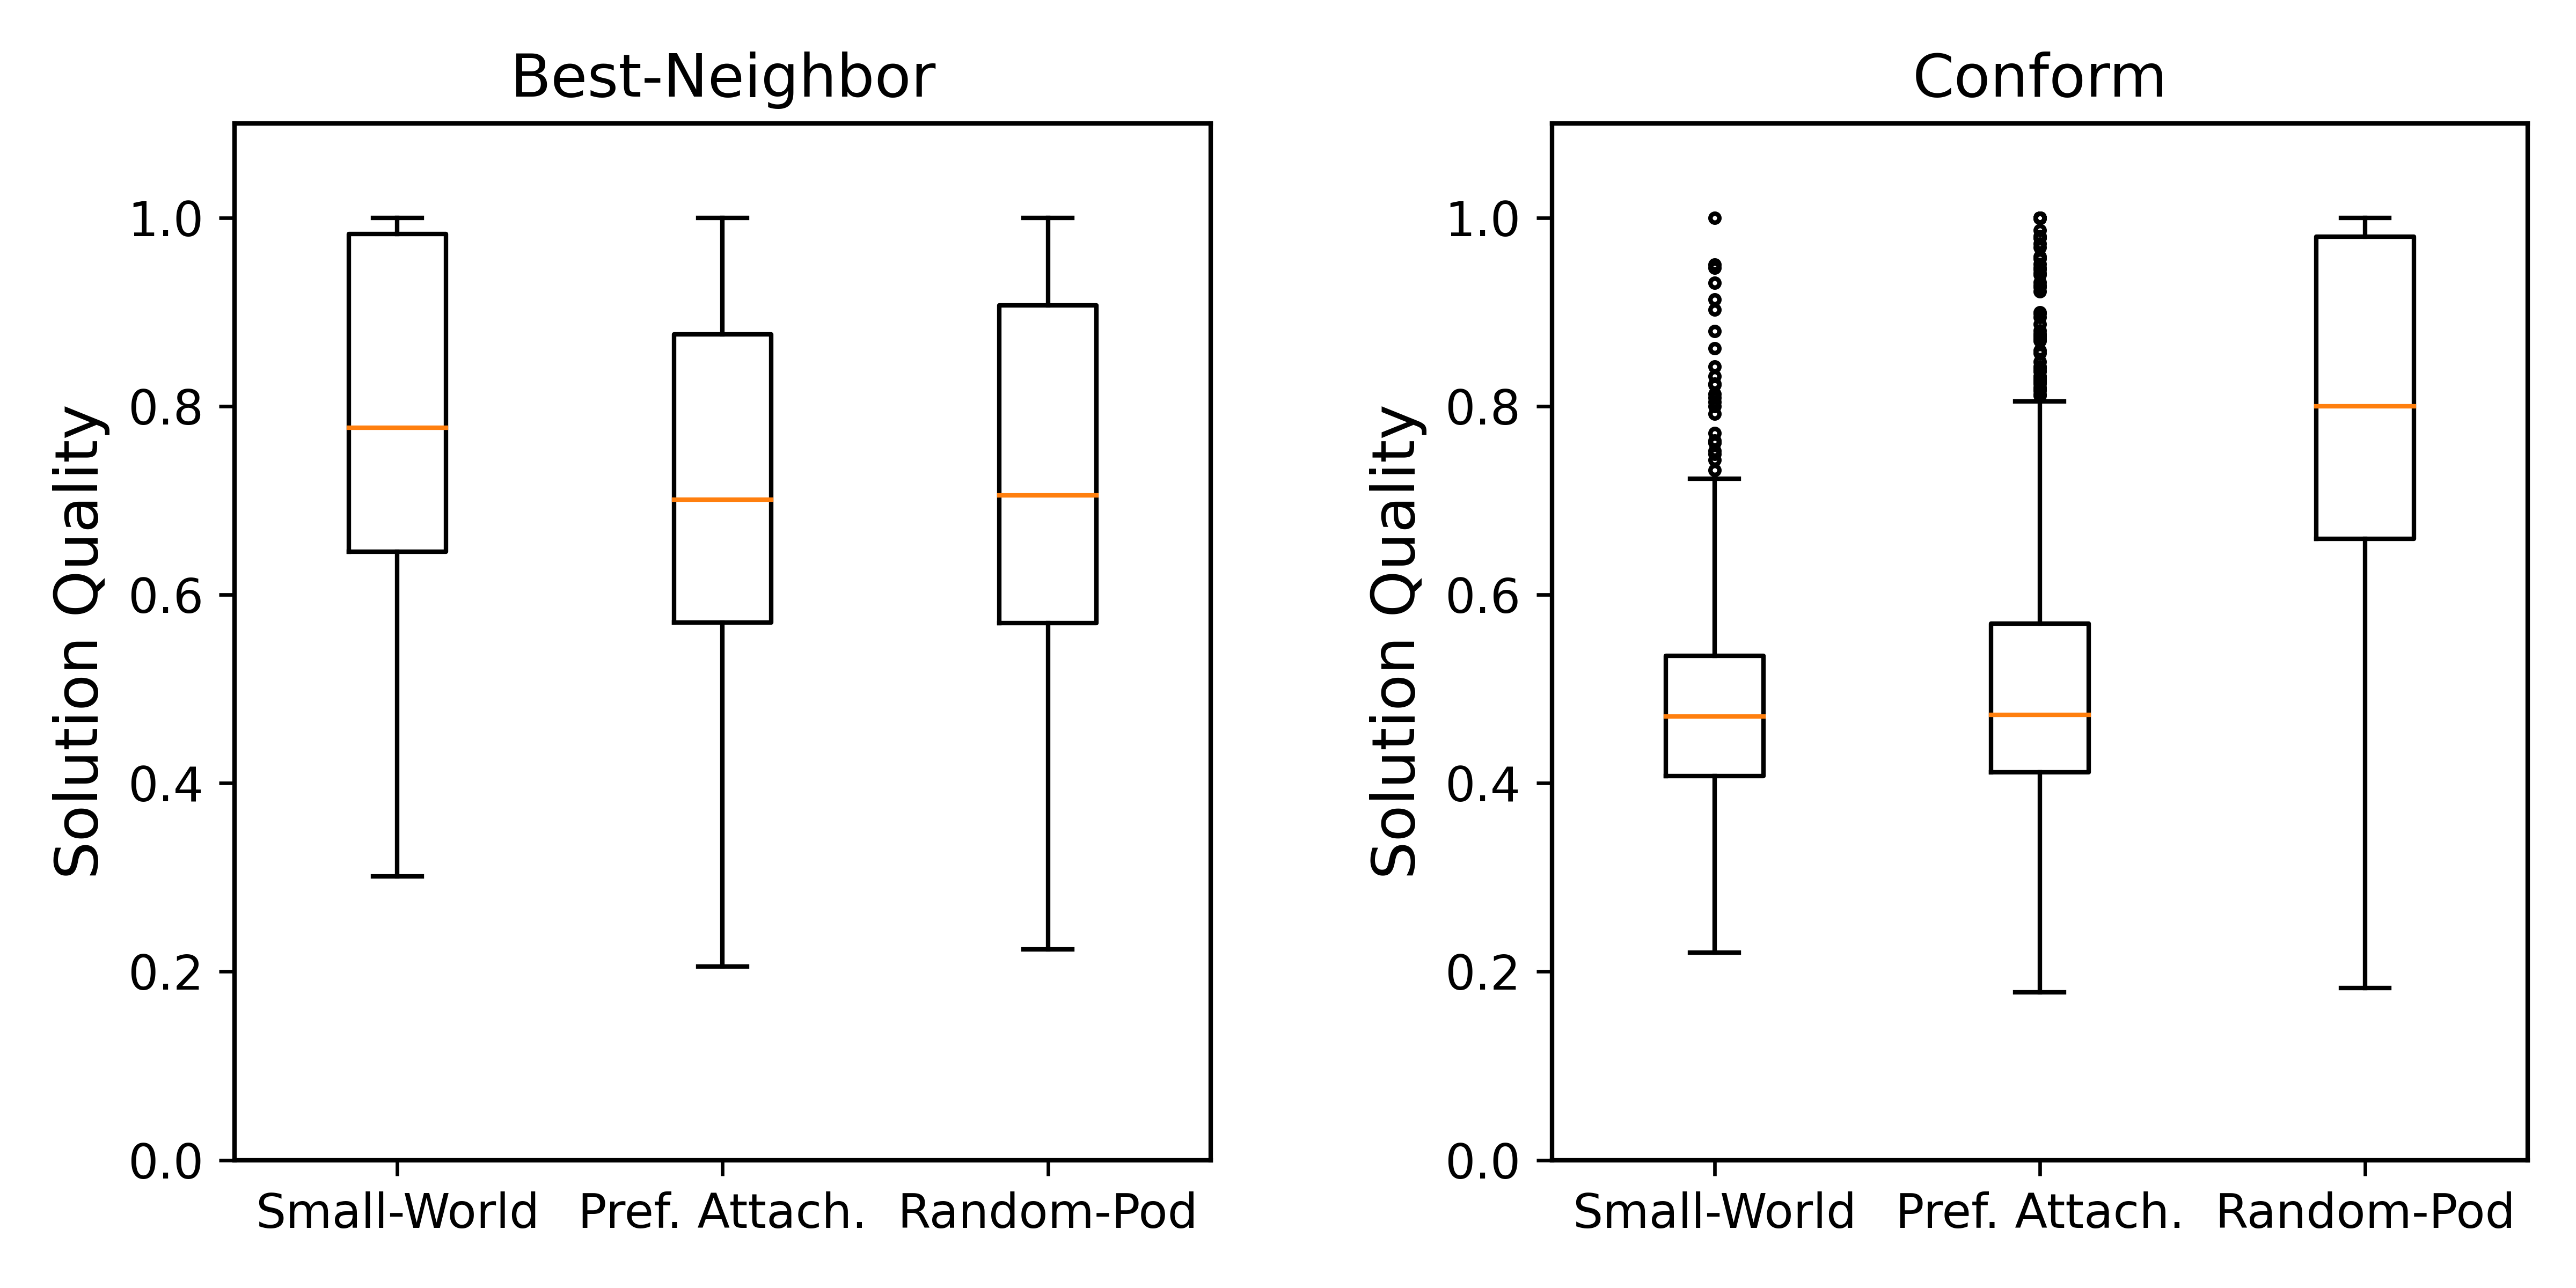
\includegraphics[width=5in]{fig-netdelib-results-net-boxplot.png}
\caption{Solution quality for 1000 runs of the agent-based model. For each run, quality is avereaged over all 100 agents.}
\label{fig:quality}
\Description[Two box plots]{The left plot shows results for the best-neighbor strategy, similar across all three networks, ranging from 0.2 to 1.0 with medians around 0.7. The right plot shows results for the conform strategy, ranging from 0.2 to 1.0. Small-world and preferential attachment have medians around 0.45, while random-pod has median about 0.8.}
\end{center}
\end{figure}

For more insight into the mechanism behind the random-pod network's
performance in the high-conformity case,
we examine the progress of the agents over the course of the simulation.
In particular, we focus on the basins of attraction associated with each agent's solution.
The basins of attraction are sets of similar solutions that all converge
to the same local maximum under a simple hill-climbing algorithm.

Figure \ref{fig:transitions} shows, on average,
how many agents switch basins of attraction at each timestep.
We further divide these transitions by whether the new basin's maximum is
higher or lower than the previous basin's.
We observe a qualitative difference between the behavior of the agents in the
random-pod network as compared to the other two networks.
In the small-world and preferential attachment networks,
the number of transitions decreases quickly, with the number of positive
transitions slightly larger than the number of negative.
For random-pod however,
the number of positive transitions remains notably higher than the number
of negative transitions.
While agents in the random-pod network are just as likely to adopt
a popular sub-optimal solution temporarily,
they more frequently continue trying new solutions until finding an
improvment.

\begin{figure}
\begin{center}
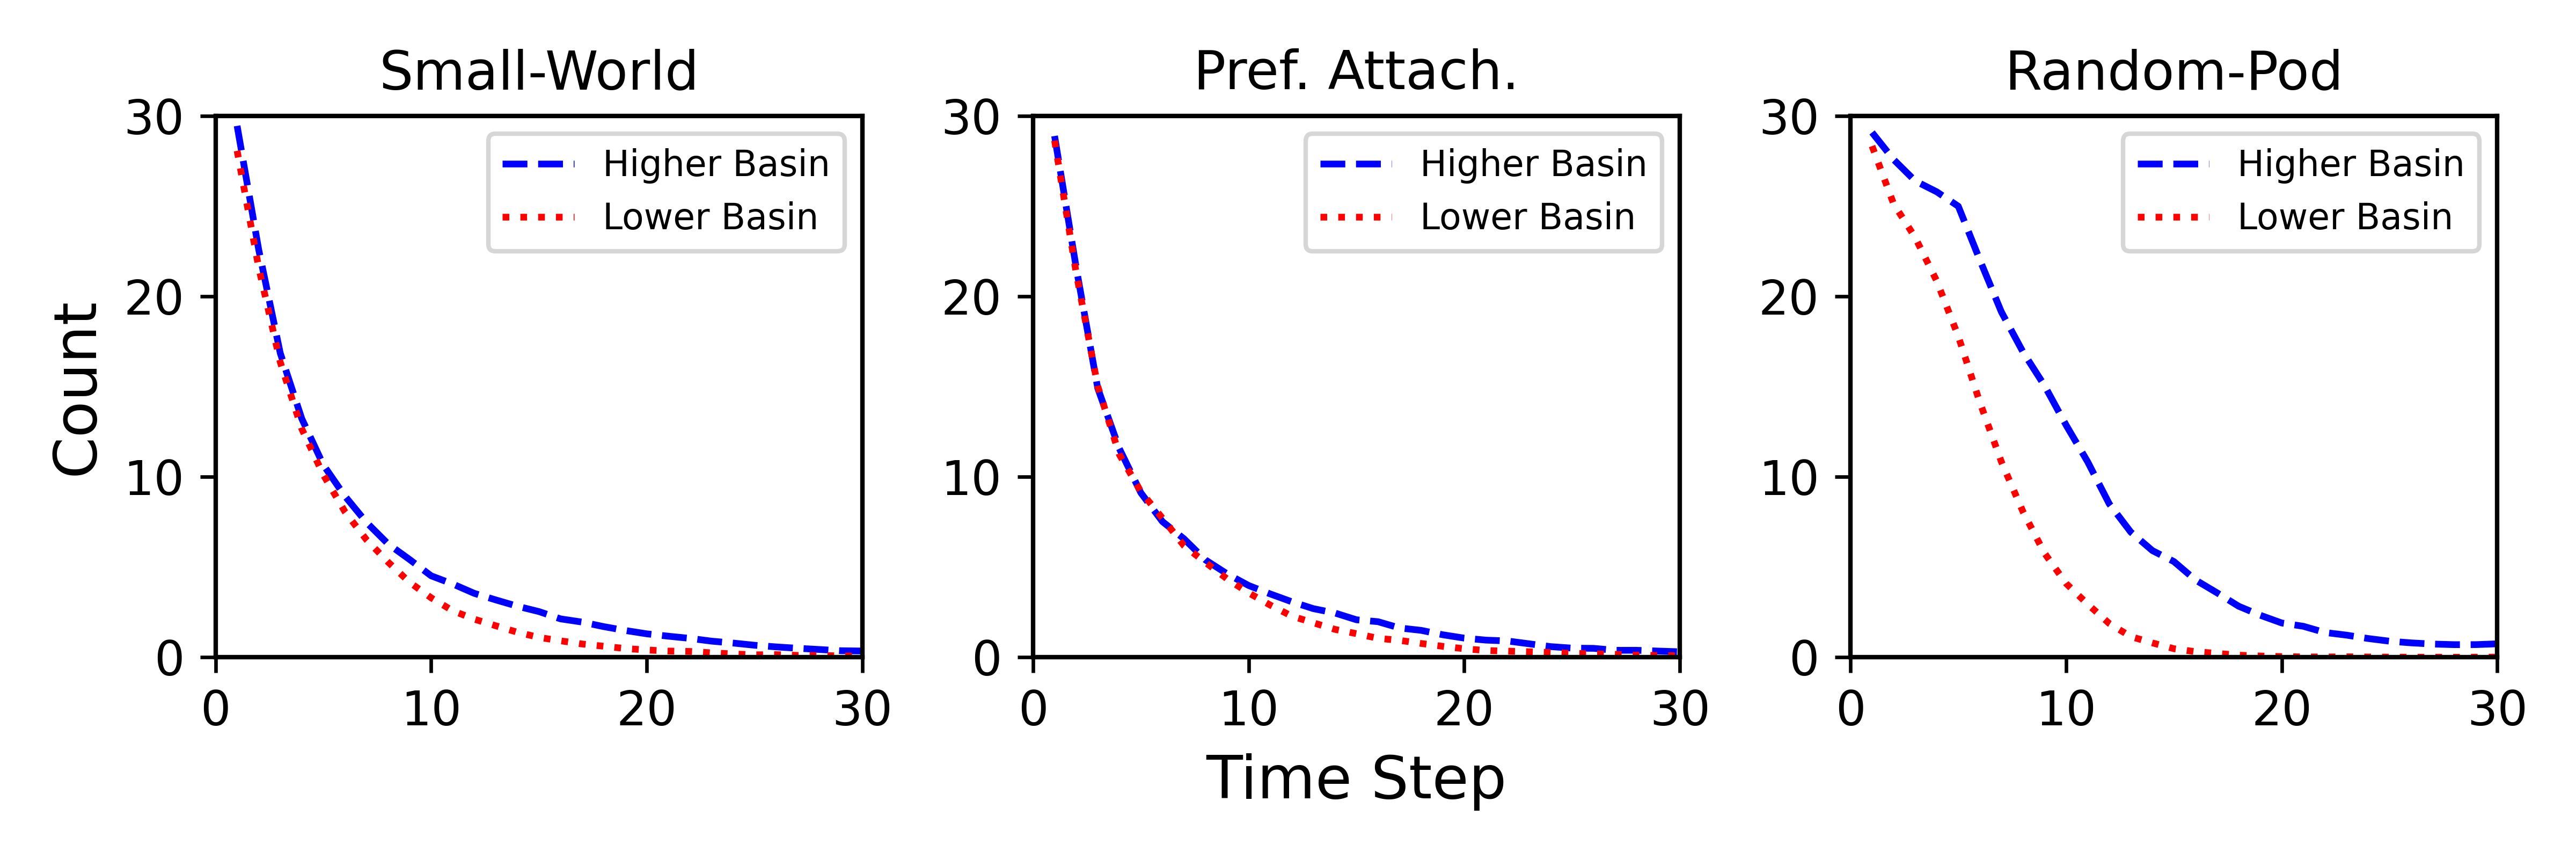
\includegraphics[width=5in]{fig-conform-transition-basin.png}
\caption{Mean number of agents adopting solutions from a different basin of attraction.}
\label{fig:transitions}
\Description[Three time-series plots, one for each network]{All plots start around 30, curve downward at different rates described in the text, and reach 0 around timestep 30.}
\end{center}
\end{figure}

\subsection{Interlocks and Convergence Speed}
Figure \ref{fig:convergence} shows the distribution of time steps necessary for agents to converge to a stable solution.
In the low-conformity best-neighbor case,
random-pod performs comparably to preferential attachment,
both of which converge slightly faster than the small-world network.
All networks converge considerably slower in the high-conformity case.
While improved performance might be expected to come at the cost of slower
speed,
the random-pod network's median convergence is actually faster than that of the other two networks.
However, the random-pod networks slowest runs are notably slower than those for the other networks.

\begin{figure}
\begin{center}
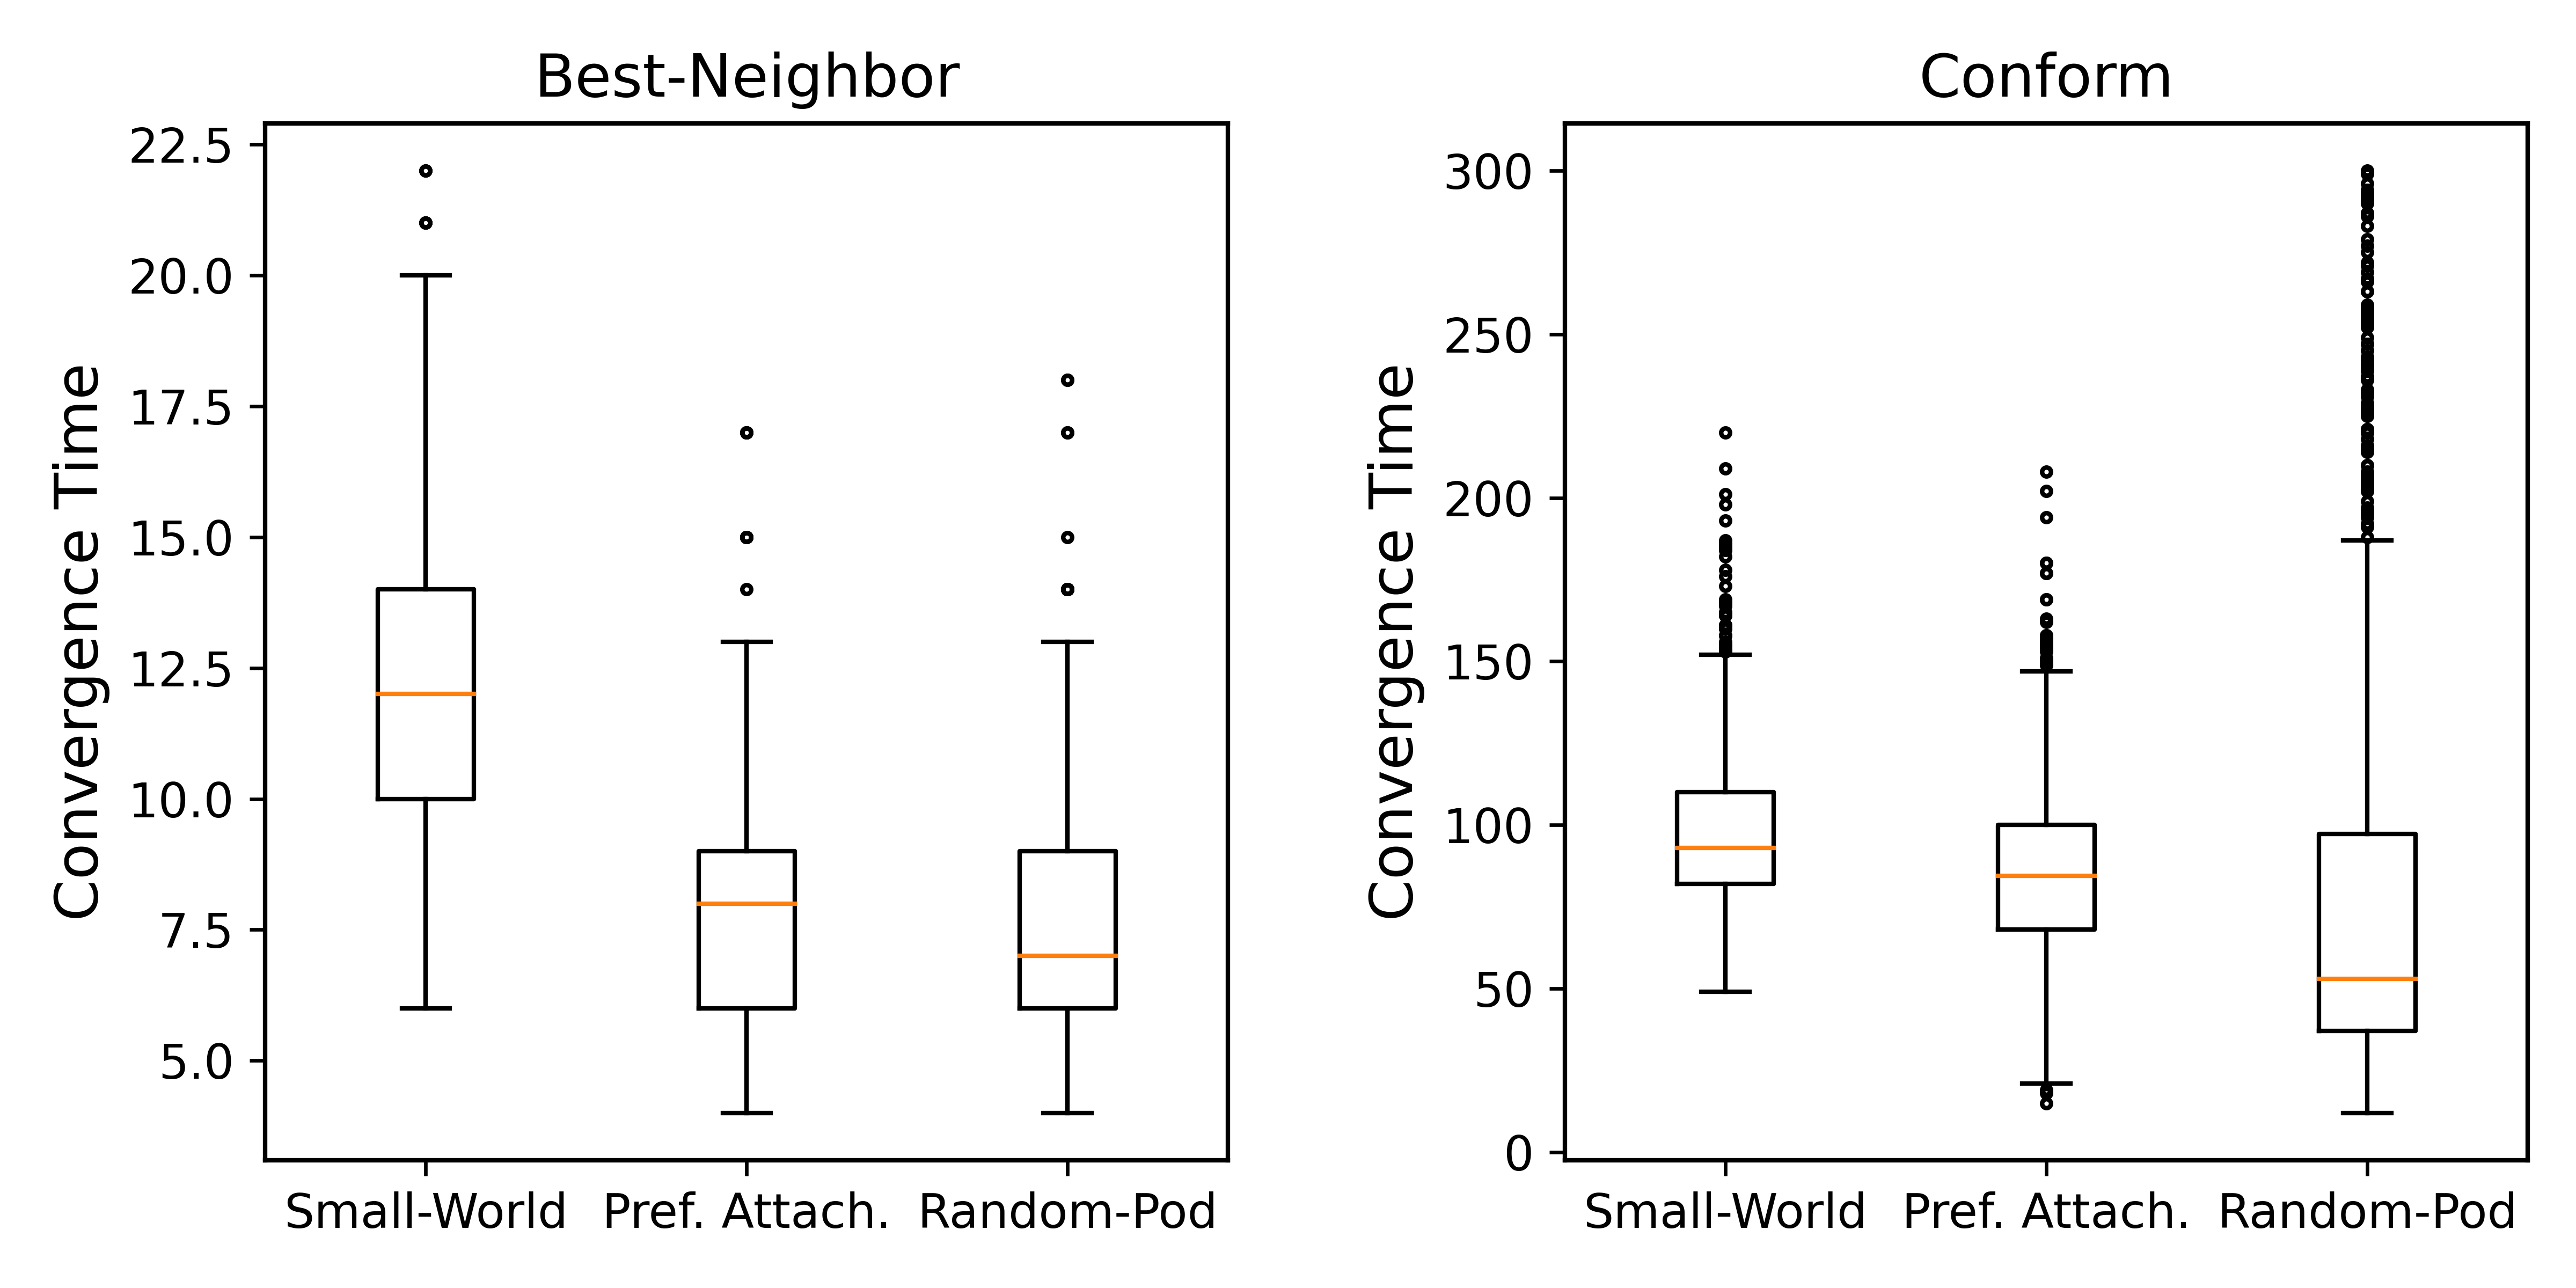
\includegraphics[width=5in]{fig-netdelib-converge-net-boxplot.png}
\caption{Distribution of convergence time for 1000 runs of the simulation.}
\label{fig:convergence}
\Description[Two box plots]{The left, for best-neighbor ranges from about 5.0 to 22.5, with more
details described in the text. The right, for conform, ranges between 0 and 300,
with more details described in the text.}
\end{center}
\end{figure}

\subsection{Interlocks and Polarization}
Figure \ref{fig:basins} shows the number of basins occupied at a given time
step, averaged over all 1000 runs of the conform strategy.
While the small-world and preferential attachment networks quickly begin to
level off and plateau at about 20 basins,
the random-pod network typically continues to converge until all agents have reached consensus on a single basin.
The small-world and preferential attachment networks thus exhibit polarization
(specifically multi-polar polarization or Balkanization),
while the random-pod network does not.
As we saw earlier in Figure \ref{fig:transitions},
the small-world and preferential attachment networks lead to a fast convergence to popular but sub-optimal solutions.
The observed polarization can be attributed to different neighborhoods within these networks converging to different sub-optimal solutions.
Thus the same mechanism that allows the random-pod network to prevent information cascades allows it to prevent polarization.

\begin{figure}
\begin{center}
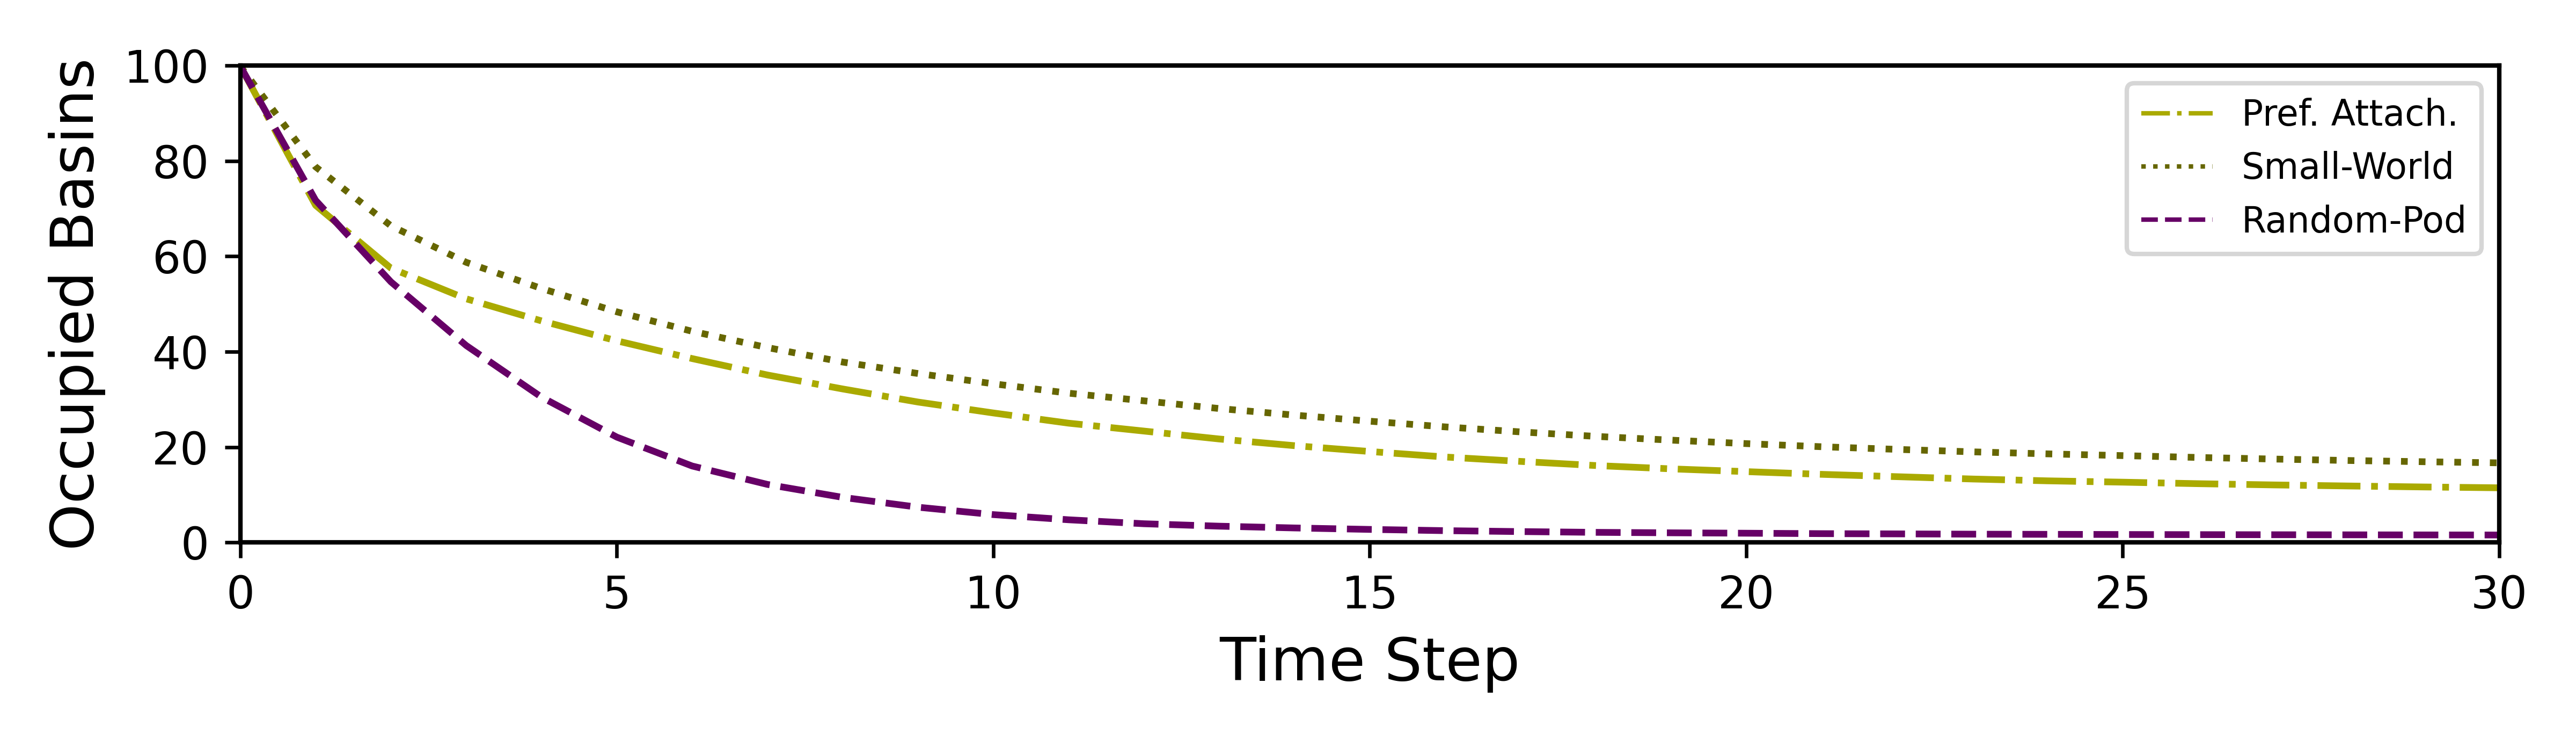
\includegraphics[width=5in]{fig-conform-basin.png}
\caption{Mean number of occupied basins of attraction over 1000 simulation runs.}
\label{fig:basins}
\Description[A time series plot]{Time ranges from time 0 to 30. Curves are shown for all three networks. Occupied basins starts at 100 and curves downward over time, with more details described in the text.}
\end{center}
\end{figure}

\section{Discussion}
We have proposed and evaluated an empirically-motivated, agent-based model of social learing,
based on the interlocking network structure observed across many successful large-scale participatory projects.
Our central finding suggests that interlocks can reduce the negative effects of conformity and social influence in social-learning,
and thereby improve deliberation and participatory governance.

Groups can exhibit conformity for a number of reasons.
Conformity can stem from social factors such as trust or social loafing.
Alternatively, conformity can supplement individual knowledge and abilities.
In the low-conformity best-neighbor strategy, we do not observe a substantial difference in output quality between the interlock network and other networks. In all cases we have looked at, interlock networks perform comparably to,
or better than other common social networks. 
Our results suggest that interlocking network structure may contribute to the success of large-scale participatory projects, and may be a useful tool for the design of large-scale sociotechnical systems.

We attribute the protective effects of interlocking network structure to its ability to stop information cascades.
A closer look at the individual agents in our model shows that conformity lowers solution quality by trapping agents in separate sub-optimal yet popular solutions and preventing them from exploring alternatives.
This outcome is consistent with the well-known phenomenon of information cascades.
In interlock networks however, a sub-optimal solution might become popular in one pod,
but members of that pod are also subject to social influence from other pods.
Those other pods are unlikely to have adopted the same sub-optimal solution,
preventing it from spreading outside its initial pod and potentially even exerting enough social influence to replace it with an improved alternative.
Similarly, by providing individuals with diverse social influence from throughout the wider network, our findings suggest interlocks can reduce polarization.

\subsection{Limitations and Future Work}
Our work is limited by several assumptions, which require further investigation to achieve greater generalizability.
We make simplifying assumptions including: a static objective function, a homogeneous strategy across all agents, and truthful agents.
All of these assumptions can be violated in some real-world settings.
We have also assumed that agents have access to the full solution string, and that agents incorporate all bits of the string into their quality estimates.
Extremely complex real-world tasks might be better-modeled by a collection of sub-tasks, with agents having access to only a subset of the solution string.
We have also limited our study to learning strategies that explore new solutions solely through small mutations of existing solutions.
Other potential strategies might generate entirely new solutions, for example, by combining parts of multiple previous solutions.
Such generative strategies would add the ability to explore a wider range of solutions. 

We also note that random assignment is just one potential way to assign pods.
Other assignment methods may create interlock networks with different properites,
such as longer mean shortest path lengths.
In fact, we have explored some other methods beyond the scope of this paper,
finding that they do alter some properties of the resulting interlock network,
but are nonetheless consistent with our present findings.

Finally, as the result of a simulation model, our findings require empirical validation.
We have conducted some initial lab experiments and interviews, which appear consistent with our findings, but further work is needed.

\subsection{Conclusion}
Our findings suggest that interlock networks, composed of small pods linked by common membership, contribute to the success of large-scale social learning and participatory decision-making, particularly when the topic is complex and social influence is strong. They do so by preventing information cascades and polarization.
These findings have implications for a range of contexts: participatory government and budgeting, worker-owned cooperatives, grassroots social movements, and the governance of decentralized technology. By enabling better and more participatory decision-making at larger scales, we hope this work will contribute to democratizing the governance of large sociotechnical systems, and empowering the individuals impacted by those systems.





%%
%% The acknowledgments section is defined using the "acks" environment
%% (and NOT an unnumbered section). This ensures the proper
%% identification of the section in the article metadata, and the
%% consistent spelling of the heading.
\begin{acks}
[redacted for peer review]
\end{acks}

%%
%% The next two lines define the bibliography style to be used, and
%% the bibliography file.
\bibliographystyle{ACM-Reference-Format}
\bibliography{references}

%%
%% If your work has an appendix, this is the place to put it.
\appendix

\section{Online Resources}
The code and data used in this paper are available online at [redacted for peer review].

\end{document}
